%----------------------------------------------------------------------------------------
%    PACKAGES AND THEMES
%----------------------------------------------------------------------------------------

\documentclass[aspectratio=169,xcolor=dvipsnames]{beamer}
\usetheme{SimplePlus}

\usepackage{hyperref}
\usepackage{graphicx} % Allows including images
\usepackage{booktabs} % Allows the use of \toprule, \midrule and \bottomrule in tables

\usepackage[caption=false]{subfig}

\usepackage{tikz}
\usetikzlibrary{positioning}

\usepackage{pgfplots}
\usepgfplotslibrary{groupplots}
\pgfplotsset{compat=1.18}

\usepackage{xspace}
\newcommand{\modelministral}{Ministral-8B\xspace}
\newcommand{\modelalpaca}{Alpaca-7B\xspace}
\newcommand{\modeldeepseek}{R1-Distill-8B\xspace}

%----------------------------------------------------------------------------------------
%    TITLE PAGE
%----------------------------------------------------------------------------------------

\title{Knowledge Graph Completion}
\subtitle{Subtitle}

\author{Eddie Groh \and Mochamad Ardiansyah Nurgaha \and Sriraam Appakutti Palani \and William Liaw}

\institute[Team: AWESome]
{
    Mehwish ALAM\\
    Associate Professor
    \and
    Language Models and Structured Data\\
}
\date{\today}

%----------------------------------------------------------------------------------------
%    PRESENTATION SLIDES
%----------------------------------------------------------------------------------------

\begin{document}

\begin{frame}
    % Print the title page as the first slide
    \titlepage
\end{frame}

% \begin{frame}{Overview}
%     \tableofcontents
% \end{frame}

%------------------------------------------------
\section{Problem Statement \& Background}
%------------------------------------------------
\begin{frame}{Problem Statement}
    \begin{block}{Knowledge Graph Completion (KGC)}
        Aims to infer missing facts in a knowledge graph (KG), represented as \( G = (E, R, T) \).
    \end{block}

    \begin{columns}[c]
        \column{.45\textwidth}
        KGC involves key tasks:
        \begin{itemize}
            \item \textbf{Link Prediction}: Identifying missing entities by ranking candidate tail entities in an incomplete triple \( (h, r, ?) \).
            \item \textbf{Triple Classification}: Determining whether a given triple \( (h, r, t) \) is valid.
        \end{itemize}
        \column{.45\textwidth}
        \\LLM-based primary approaches:
        \begin{itemize}
            \item \textbf{Prompt-Based Methods} \\(e.g., KICGPT \cite{wei2023kicgpt})\\ Utilize structured retrieval and in-context learning for entity ranking.
            \item \textbf{Fine-Tuning-Based Methods} \\(e.g., KoPA \cite{qin2023kopa})\\ Integrate structured knowledge into LLMs via additional training.
        \end{itemize}
    \end{columns}
\end{frame}

%------------------------------------------------
\section{Methodology}
%------------------------------------------------
\begin{frame}{KICGPT: Retrieval-Augmented Prompting}
    \begin{itemize}
        \item Retrieve candidate entities from the knowledge graph.
        \item Generate Knowledge Prompts for in-context learning.
        \item Perform reranking using a large language model.
    \end{itemize}
    \begin{figure}[h]
        \centering
        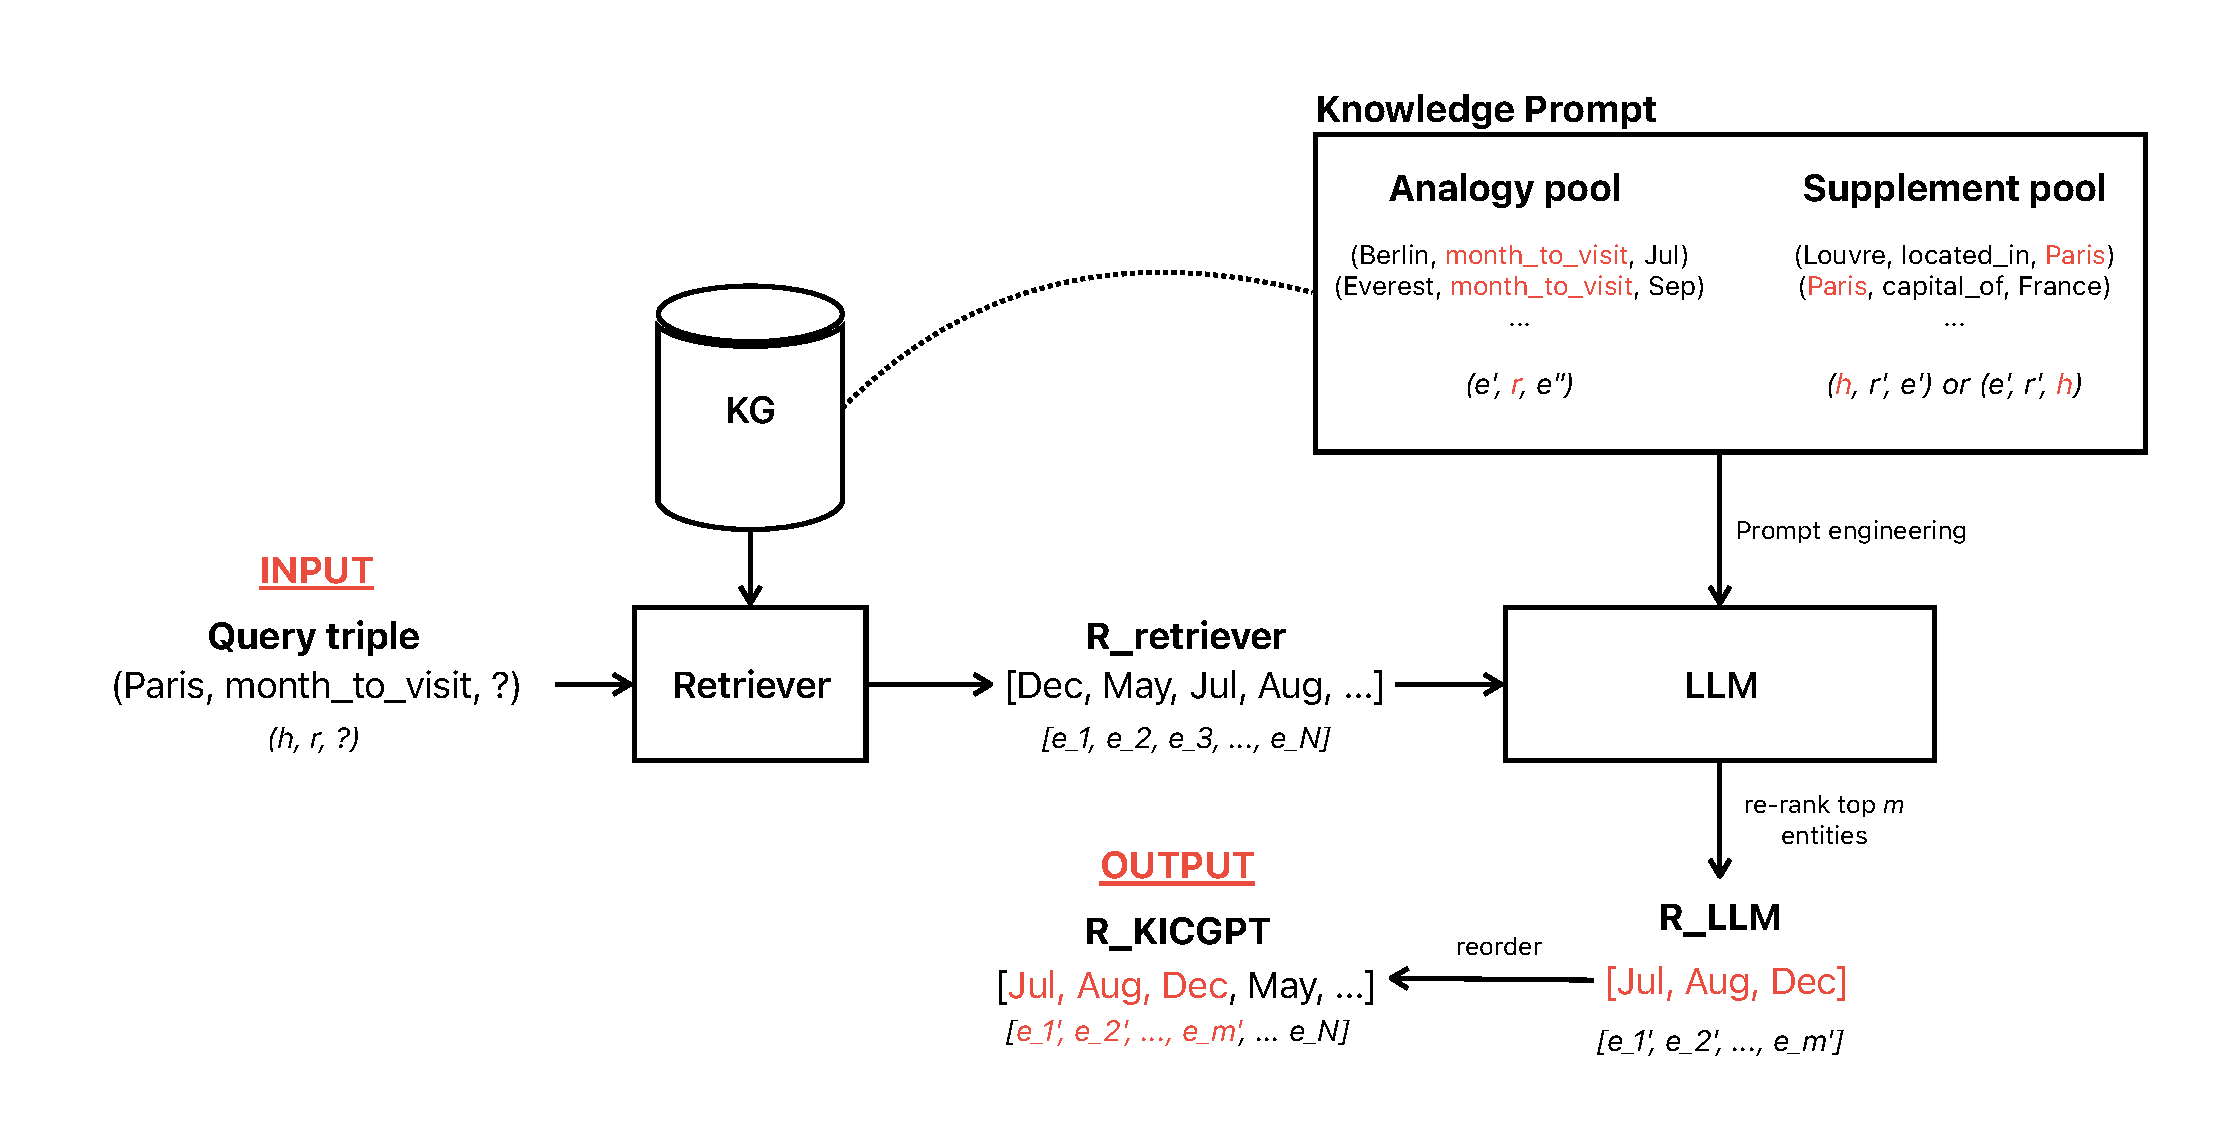
\includegraphics[width=0.8\linewidth]{images/KICGPT.pdf}
        \caption{KICGPT Architecture}
    \end{figure}
\end{frame}

\begin{frame}{KoPA: Fine-Tuning-Based Triple Classification}
    \begin{itemize}
        \item Uses Knowledge Prefix Adapter (KPA) to integrate KG structure.
        \item Embeddings guide LLM reasoning.
        \item Fine-tuned LLM predicts validity of triples.
    \end{itemize}
    \begin{figure}[h]
        \centering
        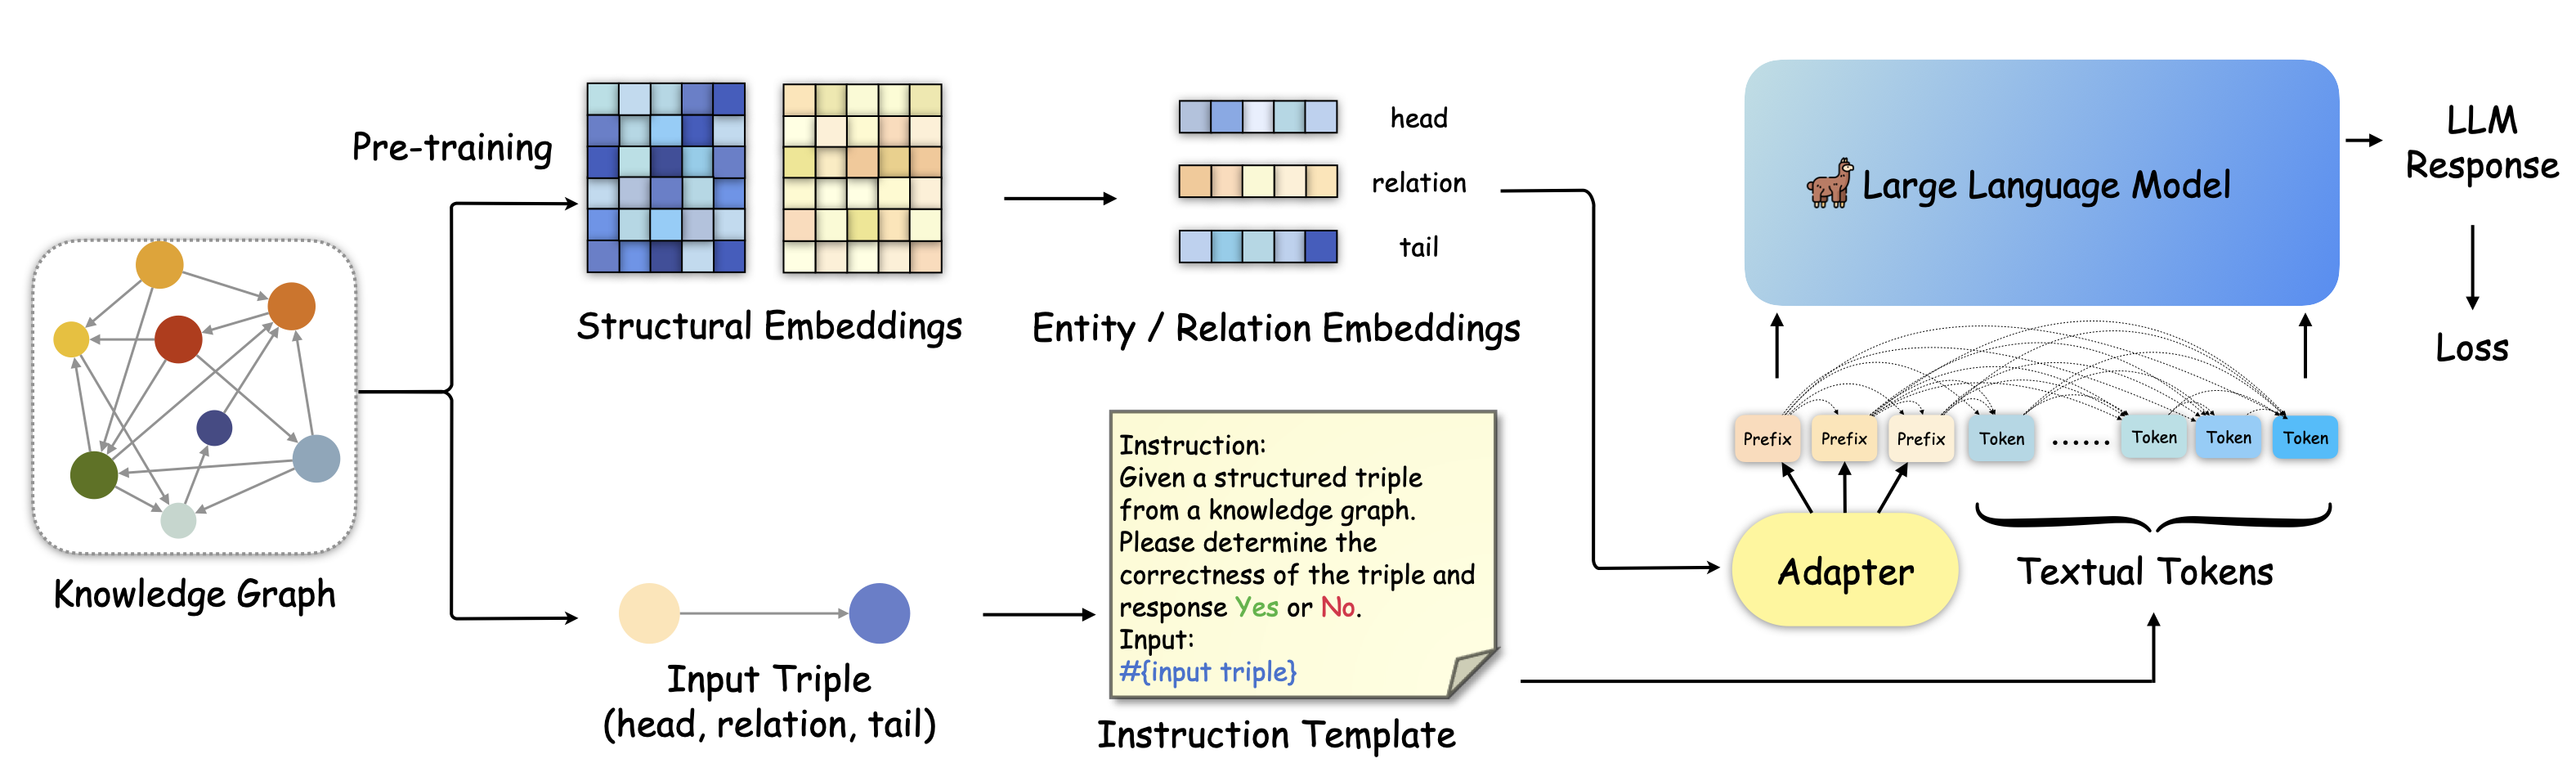
\includegraphics[width=0.8\linewidth]{images/KoPAarchitecture.png}
        \caption{KoPA Architecture}
    \end{figure}
\end{frame}


%------------------------------------------------
\section{Experiments \& Discussion}
%------------------------------------------------
\begin{frame}{Experiments}
    \begin{columns}[c]
        \column{.45\textwidth}
        Datasets: WN18RR and CoDeX-S.
        \begin{table}[h]
            \centering
            \begin{tabular}{l c c c c c}
                \toprule
                \textbf{Dataset} & \textbf{\# Entities} & \textbf{\# Relations} \\
                \midrule
                WN18RR           & 40,943               & 11                    \\
                CoDeX-S          & 2,034                & 42                    \\
                \bottomrule
            \end{tabular}
            \caption{Statistics of the datasets used in our experiments.}
            \label{tab:datasets}
        \end{table}

        \column{.45\textwidth}
        LLMs Compared:
        \begin{itemize}
            \item \textbf{\modelalpaca} – Fine-tuned for \textit{instruction-following} tasks.
            \item \textbf{\modelministral} – Optimized for \textit{multilingual and long-context} scenarios.
            \item \textbf{\modeldeepseek} – A distilled model with strong \textit{reasoning} capabilities.
        \end{itemize}
    \end{columns}
\end{frame}

\begin{frame}{Plots}
    \begin{columns}[c]
        \column{.45\textwidth}
        Retrieval-Augmented Prompting
        \begin{figure}[ht]
            \centering
            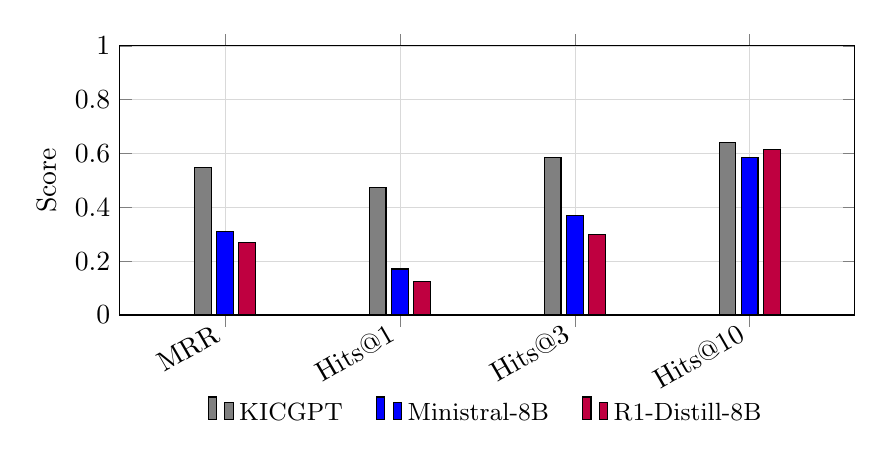
\begin{tikzpicture}
                \begin{axis}[
                        ybar,
                        bar width=6pt,
                        symbolic x coords={MRR, Hits@1, Hits@3, Hits@10},
                        xtick=data,
                        xticklabel style={rotate=30, anchor=east},
                        ymin=0,
                        ymax=1,
                        ylabel={Score},
                        width=0.9\textwidth,
                        height=5cm,
                        grid=both,
                        major grid style={line width=.2pt, draw=gray!30},
                        minor grid style={draw=gray!10},
                        enlarge x limits=0.2,
                        % Legend placed below with spacing:
                        legend style={
                                at={(0.5,-0.28)},
                                anchor=north,
                                /tikz/every even column/.append style={column sep=10pt},
                                legend columns=3,
                                draw=none, % Remove box
                                fill=none,
                                font=\small
                            }
                    ]

                    % Bars
                    \addplot[fill=gray]   coordinates {(MRR,0.549)  (Hits@1,0.474)  (Hits@3,0.585)  (Hits@10,0.641)};
                    \addlegendentry{KICGPT}
                    \addplot[fill=blue]   coordinates {(MRR,0.3112) (Hits@1,0.1707) (Hits@3,0.3711) (Hits@10,0.5862)};
                    \addlegendentry{\modelministral}
                    \addplot[fill=purple] coordinates {(MRR,0.2700) (Hits@1,0.1233) (Hits@3,0.2994) (Hits@10,0.6145)};
                    \addlegendentry{\modeldeepseek}

                \end{axis}
            \end{tikzpicture}
            \caption{Link Ordering Evaluation Metrics}
            \label{fig:link_ordering}
        \end{figure}

        \column{.45\textwidth}
        Fine-Tuning-Based Triple Classification
        \begin{figure}[ht]
            \centering
            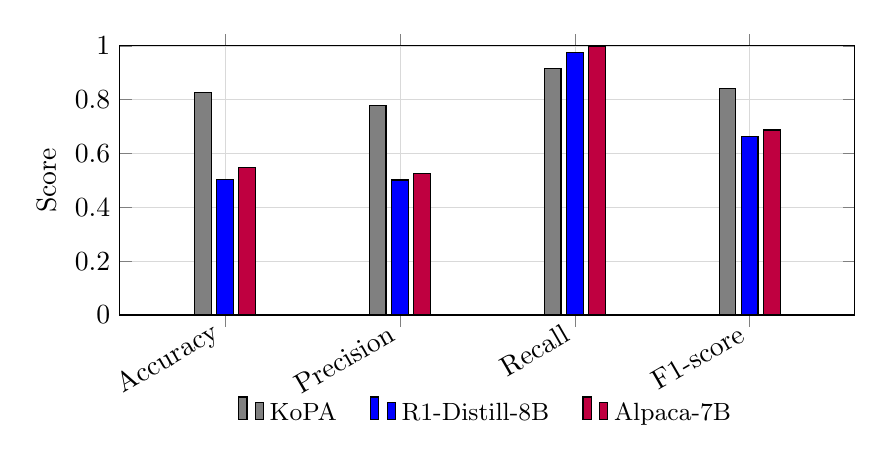
\begin{tikzpicture}
                \begin{axis}[
                        ybar,
                        bar width=6pt,
                        symbolic x coords={Accuracy, Precision, Recall, F1-score},
                        xtick=data,
                        xticklabel style={rotate=30, anchor=east},
                        ymin=0,
                        ymax=1,
                        ylabel={Score},
                        width=0.9\textwidth,
                        height=5cm,
                        grid=both,
                        major grid style={line width=.2pt, draw=gray!30},
                        minor grid style={draw=gray!10},
                        enlarge x limits=0.2,
                        legend style={
                                at={(0.5,-0.28)},
                                anchor=north,
                                /tikz/every even column/.append style={column sep=10pt},
                                legend columns=3,
                                draw=none,
                                fill=none,
                                font=\small
                            }
                    ]

                    % Bars
                    \addplot[fill=gray]   coordinates {(Accuracy,0.8274)  (Precision,0.7791)  (Recall,0.9141)  (F1-score,0.8411)};
                    \addlegendentry{KoPA}

                    \addplot[fill=blue]   coordinates {(Accuracy,0.5027) (Precision,0.5014) (Recall,0.9759) (F1-score,0.6625)};
                    \addlegendentry{\modeldeepseek}

                    \addplot[fill=purple] coordinates {(Accuracy,0.5465) (Precision,0.5245) (Recall,0.9962) (F1-score,0.6872)};
                    \addlegendentry{\modelalpaca}
                \end{axis}
            \end{tikzpicture}
            \caption{CoDeX Performance Evaluation Metrics}
            \label{fig:codex_evaluation}
        \end{figure}

    \end{columns}
\end{frame}

\begin{frame}{Plots}
    \begin{figure}
        \centering
        \begin{tikzpicture}
            % Group plot configuration
            \begin{groupplot}[
                    group style={
                            group size=3 by 1,       % 3 plots in 1 row
                            horizontal sep=0.3cm     % Adjust spacing between plots
                        },
                    width=0.3\textwidth,         % Maximized plot width
                    ymode=log,                   % Log-scale y-axis for ALL plots
                    xmin=0, xmax=3,              % Unified x-axis range
                    ymin=1e-3, ymax=1,           % Unified y-axis range across all plots
                    xlabel=Epoch,
                    xtick distance=0.5,          % Uniform tick spacing
                    ytick distance=10,           % Log-scale tick separation
                    minor y tick num=9,          % Minor tick marks for readability
                ]

                %------------- Plot (a) Alpaca -----------------
                \nextgroupplot[
                    title=\modelalpaca,
                    % Hide y-axis labels for alignment
                    ylabel=Loss
                ]
                \addplot[smooth, thick, blue]
                table[x=epoch, y=loss, col sep=space]
                    {images/raw-data/lora-Llama-2-7b-alpaca-cleaned-finetune.dat};

                \addplot[smooth, thick, cyan, dashed]
                table[x=epoch, y=grad-norm, col sep=space]
                    {images/raw-data/lora-Llama-2-7b-alpaca-cleaned-finetune.dat};


                %------------- Plot (b) DeepSeek ---------------
                \nextgroupplot[
                    title=\modeldeepseek,
                    yticklabels={,,}
                ]
                \addplot[smooth, thick, purple]
                table[x=epoch, y=loss, col sep=space]
                    {images/raw-data/lora-DeepSeek-R1-Distill-Llama-8B-finetune.dat};

                \addplot[smooth, thick, violet, dashed]
                table[x=epoch, y=grad-norm, col sep=space]
                    {images/raw-data/lora-DeepSeek-R1-Distill-Llama-8B-finetune.dat};

                %------------- Plot (c) Loss Comparison -------------
                \nextgroupplot[
                    title=Loss Comparison,
                    yticklabels={,,}   % Hide y-axis tick labels for uniform look
                ]
                \addplot[smooth, thick, purple]
                table[x=epoch, y=loss, col sep=space]
                    {images/raw-data/lora-DeepSeek-R1-Distill-Llama-8B-finetune.dat};

                \addplot[smooth, thick, blue]
                table[x=epoch, y=loss, col sep=space]
                    {images/raw-data/lora-Llama-2-7b-alpaca-cleaned-finetune.dat};

            \end{groupplot}
        \end{tikzpicture}

        % Description of colors with more spacing in legend
        \vspace{0.2cm}
        {\centering
            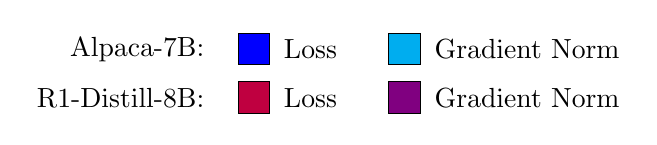
\begin{tikzpicture}
                \node[draw, fill=blue, minimum width=0.4cm, minimum height=0.4cm] (A) {};
                \node[left=0.3cm of A] {\modelalpaca:};
                \node[right=0.05cm of A] {Loss};

                \node[draw, fill=cyan, minimum width=0.4cm, minimum height=0.4cm, right=1.5cm of A] (B) {};
                \node[right=0.05cm of B] {Gradient Norm};

                \node[draw, fill=purple, minimum width=0.4cm, minimum height=0.4cm, below=0.2cm of A] (C) {};
                \node[left=0.3cm of C] {\modeldeepseek:};
                \node[right=0.05cm of C] {Loss};

                \node[draw, fill=violet, minimum width=0.4cm, minimum height=0.4cm, right=1.5cm of C] (D) {};
                \node[right=0.05cm of D] {Gradient Norm};
            \end{tikzpicture}
        }

        \caption{Fine-tuning of \modelalpaca and \modeldeepseek. Loss and gradient norm trends are shown separately for each model, along with a comparison of both losses. Figure and results from our work.}
        \label{fig:training_comparison}
    \end{figure}
\end{frame}

\begin{frame}{Discussion}
    TBD
\end{frame}

%------------------------------------------------
\section{Conclusion}
%------------------------------------------------
\begin{frame}{Conclusion}
    TBD
\end{frame}

\begin{frame}{References}
    \footnotesize
    \bibliography{reference.bib}
    \bibliographystyle{apalike}
\end{frame}

\end{document}
